\documentclass[12pt,a4paper]{report}
\usepackage[utf8]{inputenc} % un package
\usepackage[T1]{fontenc} % un second package
\usepackage[francais]{babel} % un troisième package
\usepackage{color} % Package de la couleur
\usepackage{verbatim}
\usepackage{moreverb}
\usepackage{amsmath}
\usepackage{amsfonts}
\usepackage{amssymb}
\usepackage{graphicx}
\usepackage[top=2cm, bottom=2cm, left=2cm, right=2cm]{geometry}
\author{IMA World Health Web Developer Team}
\title{
\includegraphics[width=12cm]{ima.png} \\Hospital Management System\\ (HMS) \\ Manuel d'utilisation}

\begin{document}
%Page de garde
\maketitle 
\chapter{Présentation}
\section{Accès au système}
\large{Pour accéder au système, la première de chose à faire est de lancer un navigateur web, en suite saisir l'adresse web de l'application dans la barre d'adresse du navigateur.}

La première interface de l'application est un formulaire qui demande à chaque utilisateur de pouvoir fournir le login, le mot de passe mais  aussi le projet dont il sont assigné, comme le montre le formulaire ci-dessous.
\begin{figure}[h]
\begin{center}
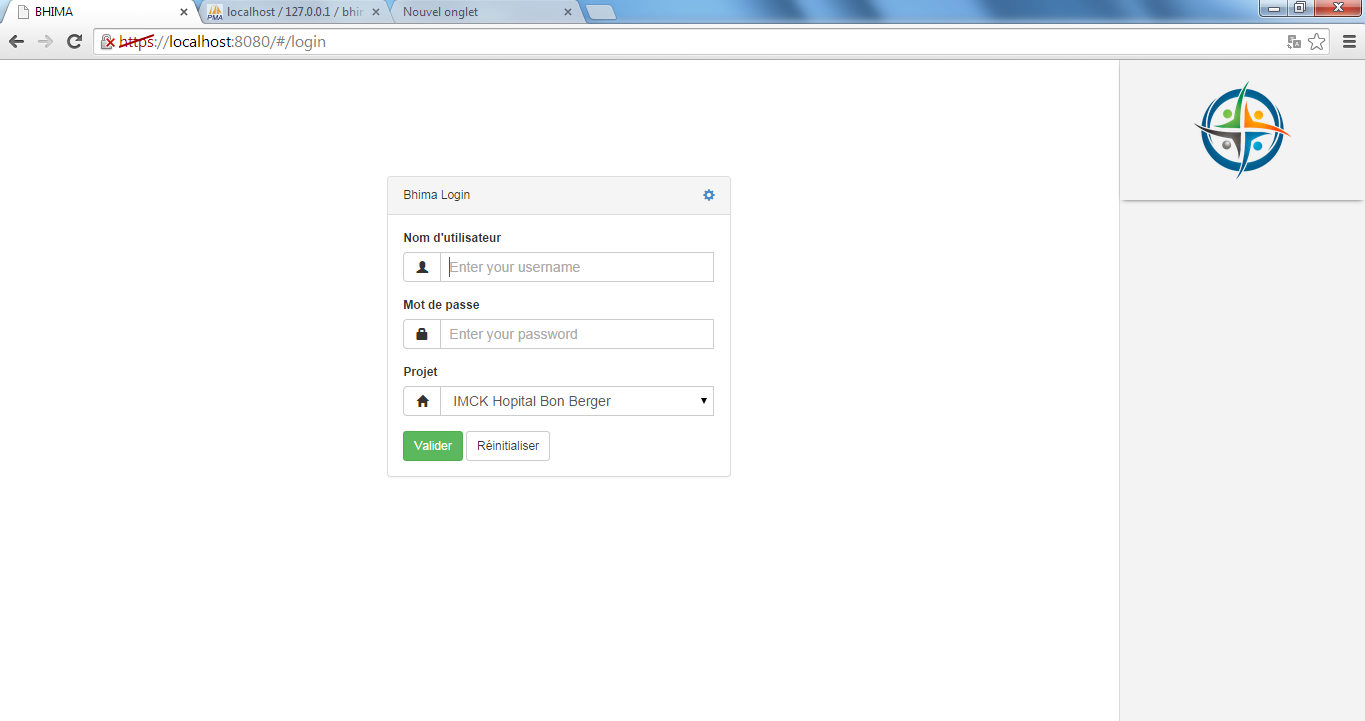
\includegraphics[width=12cm]{pic/login.png}
\end{center}
\caption{Page d'identification et authentification des utilisateurs}
\label{Page d'identification et authentification des utilisateurs}
\end{figure}
\\ L'accès au système n'est garanti que pour ceux qui possèdent un compte utilisateur, si l'utilisateur est authentifié alors il sera dirigé vers l'interface principale de l'application qui se présente de la manière suivante.
\newpage
\begin{figure}[h]
\begin{center}
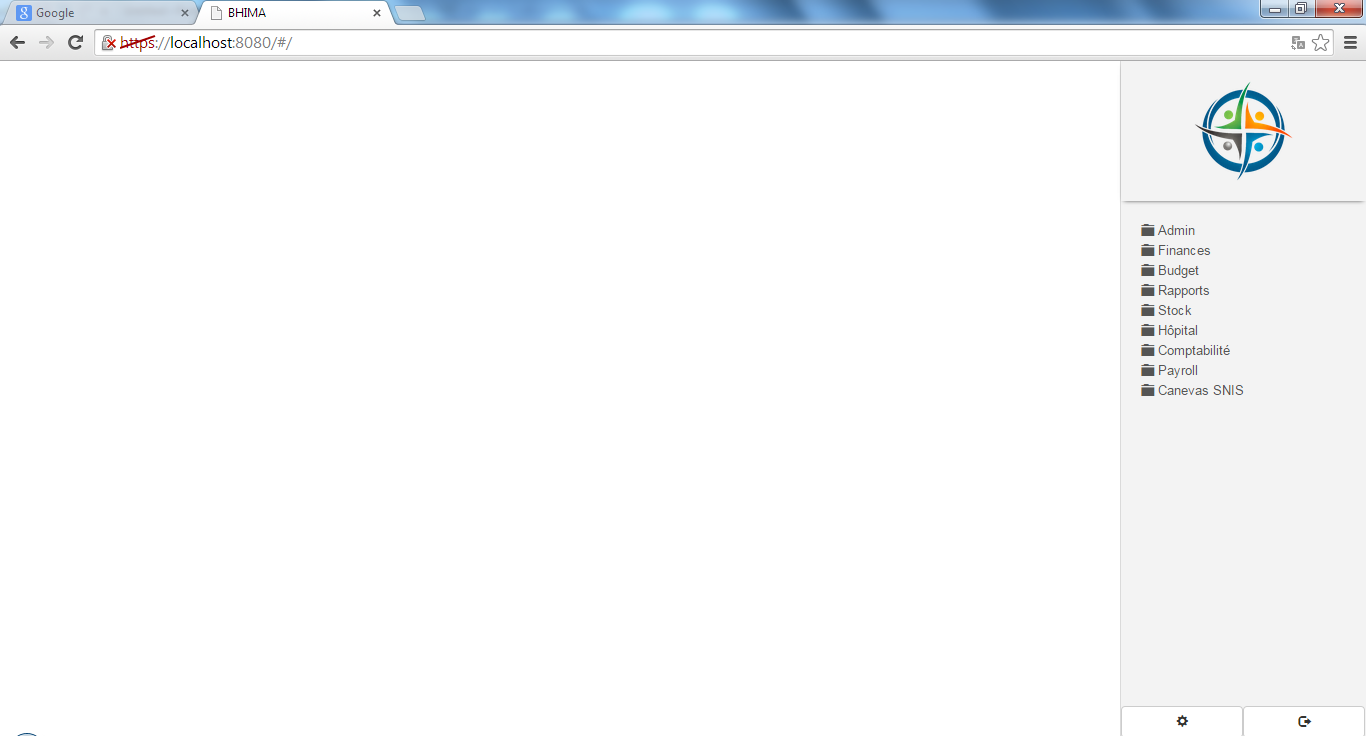
\includegraphics[width=10cm]{pic/mainInterface.png}
\end{center}
\caption{Interface principale de l'application}
\label{Interface principale de l'application}
\end{figure} 
Dans sa partie gauche de la figure ci-dessous on retrouve le logo IMA World Heath Ainsi que l'arborescence qui représente le niveau d'accès de l'utilisateur. En dessous de l'arborescence figure deux boutons, le premier 
\includegraphics[scale=0.5]{pic/lang.png} permet de changer de langue et le second 
\includegraphics[scale=0.5]{pic/logout.png} permet de ce déconnecté du système.

\begin{figure}[h]
\begin{center}
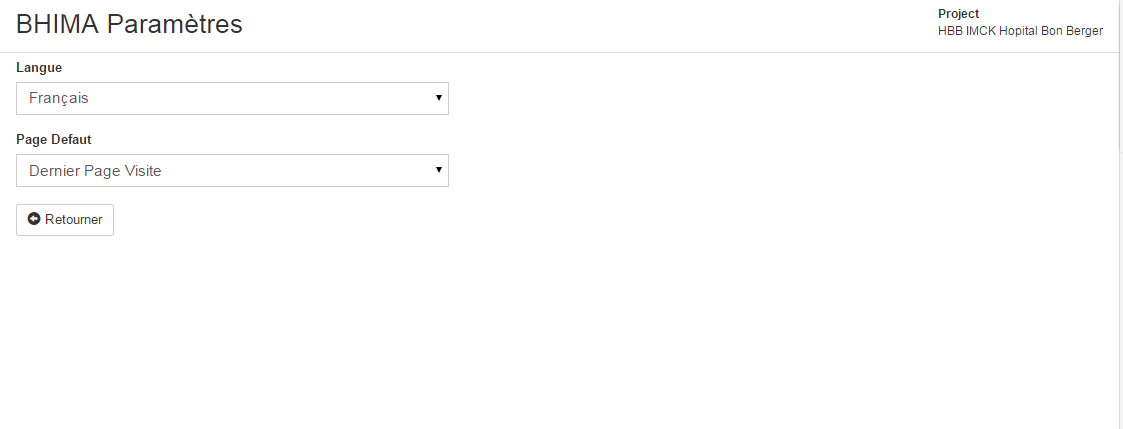
\includegraphics[width=10cm]{pic/changeLang.png}
\end{center}
\caption{Interface principale pour le changement de langue}
\label{Interface principale pour le changement de langue}
\end{figure} 
\newpage
\section{Les modules du système HMS}
Le système d'information HMS possède plusieurs modules qui sont représenté par l'arborescence ci-dessous.
\begin{figure}[h]
\begin{center}
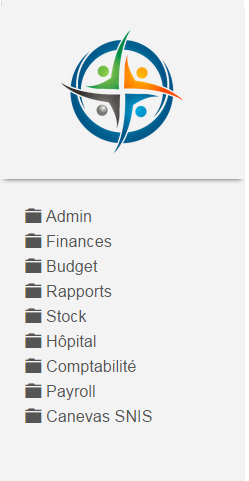
\includegraphics[width=4.5cm]{pic/arbo.png}
\end{center}
\caption{Arborescence du système}
\label{Arborescence du système}
Voici les différentes rubriques qui existent dans le système:
\end{figure} 
% Liste des modules
\begin{itemize}
\item Admin. %•
\item Finance
\item Budget
\item Rapports
\item Stock
\item Hôpital
\item Payroll
\item Comptabilité
\item Canevas SNIS
\end{itemize}
Nous allons à présent détailler chacun d'entre eux.
\newpage
%%%%%%%%%%%%%%%%%%%%%%%%%%%%%%%%%%%%%%%%%%%%%
%   MODULES DU SYSTEMES                     %
%%%%%%%%%%%%%%%%%%%%%%%%%%%%%%%%%%%%%%%%%%%%%
    
\chapter{Le module Admin}        
%////////////////////////////////////////////////%
% MODULE ADMIN
Le module admin est compose des sous modules qui permettent d'administrer le système. La figure ci-dessous représente avec exactitude ce module avec les différents sous éléments.
\begin{figure}[h]
\begin{center}
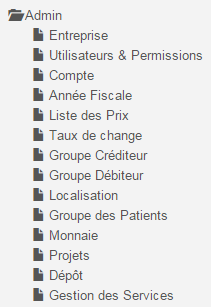
\includegraphics[width=4cm]{pic/s_admin.png}
\end{center}
\caption{Le module Admin et ses sous modules}
\label{Le module Admin et ses sous menus}
\end{figure} 


\section{Taux d'échange}
Le module de taux de change, donne la possibilité de définir le taux d'échange du jour. Par souci d'intégrité des données, Le taux d'échange doit être défini chaque jour.


\begin{figure}[h]
\begin{center}
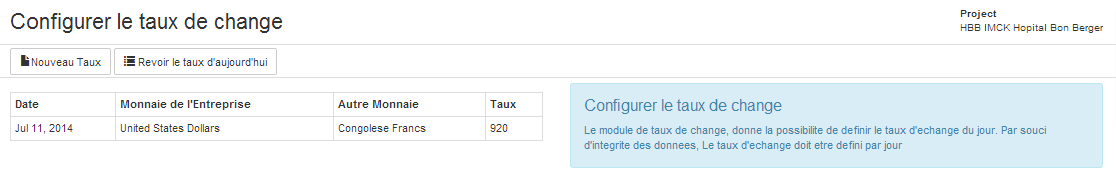
\includegraphics[width=16cm]{pic/FormulaireConfigRate.png}
\end{center}
\caption{Formulaire permettant de configurer le taux de change}
\label{Formulaire permettant de configurer le taux de change}
\end{figure}

\subsection{Nouveau Taux}
Lorsque l'utilisateur click sur le bouton 
\includegraphics[scale=0.7]{pic/NouveauTaux.png}
 Le formulaire ci-après apparait.

\begin{figure}[h]
\begin{center}
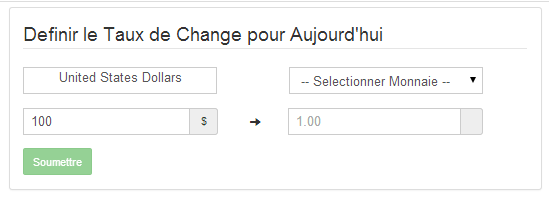
\includegraphics[width=12cm]{pic/DefinirTaux.png}
\end{center}
\caption{Formulaire permettant de definir le taux}
\label{Formulaire permettant de definir le taux}
\end{figure}
\begin{itemize}
\item \textbf{United States Dollars}: est la monnaie principale de l'application, l'équivalence avec les autres monnaie ne doit se faire qu'avec la somme de 100 Dollars,
\item \textbf{Sélectionner Monnaie}: Affiche la liste des monnaies qui existe dans le système et la zone de saisie qui se retrouve en bas permet de préciser l'équivalence avec la monnaie principale.
\end{itemize}
Après avoir renseigné ce deux champs, un clique sur le bouton \textbf{Soumettre} permet de définir les taux du jour.

\subsection{Revoir le taux d'aujourd'hui}
Un clic sur le bouton 
\includegraphics[scale=0.7]{pic/RevoirTaux.png} permet d'afficher toutes les informations sur le taux du jour, comme la montre la figure ci-dessous.
\begin{figure}[h]
\begin{center}
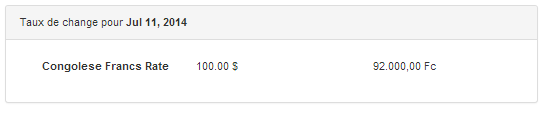
\includegraphics[width=12cm]{pic/ShowRate.png}
\end{center}
\caption{Aperçue du taux du jour}
\label{Aperçue du taux du jour}
\end{figure}
\newpage

\newpage
\chapter{Le module finance}        
%////////////////////////////////////////////////%
Le module finance est composé des sous modules qui permettent d'administrer le finance. La figure ci-dessous représente avec exactitude ce module avec ses différents sous éléments.

\begin{figure}[h]
\begin{center}
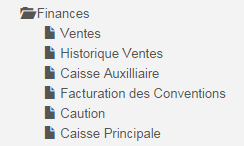
\includegraphics[width=6cm]{pic/FinanceArbo.png}
\end{center}
\caption{Arborescence du module Finance}
\label{Arborescence du module Finance}
\end{figure}


\section{Historique des ventes}
L'historique de vente permet de connaitre l'historique des toutes les opérations liée à la vente dans le système, son interface principale se présente de cette façon.


\begin{figure}[h]
\begin{center}
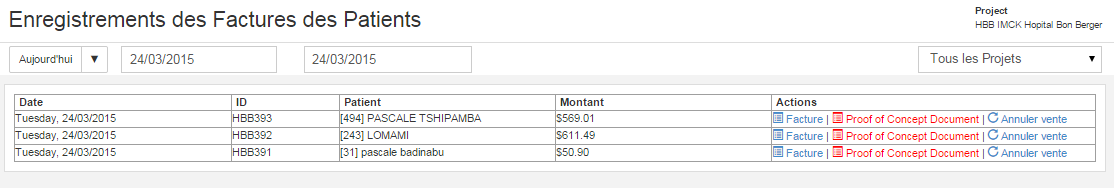
\includegraphics[width=14cm]{pic/HistoVente.png}
\end{center}
\caption{Interface principale du module Historique des ventes}
\label{Interface principale du module Historique des ventes}
\end{figure}

Les données qui se présente par défaut et celui du jour en cours mais il y'a la possibilité le modifie soit en sélectionnant dans la liste de choix, un autre critère d'affichage, sur cette liste de choix comme le montre la figure ci-après, on a le choix \textbf{entre Aujourd'hui, Cette semaine et ce mois} 


\begin{figure}[h]
\begin{center}
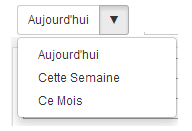
\includegraphics[width=4cm]{pic/SelectJour.png}
\end{center}
\caption{Aperçue de l'option permettant de rechercher une période de vente}
\label{Aperçue de l'option permettant de rechercher une période de vente}
\end{figure}

Mais juste à côté de cette liste de choix, on a la possibilité de préciser une plage de valeur en précisant pour ce cas la date initiale et la date terminale.

\begin{figure}[h]
\begin{center}
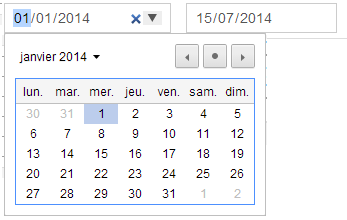
\includegraphics[width=8cm]{pic/SelectPlageValeur.png}
\end{center}
\caption{Aperçue de l'option permettant de rechercher l'historique des ventes dans une plage de temps}
\label{Aperçue de l'option permettant de rechercher l'historique des ventes dans une plage de temps}
\end{figure}

Le tableau de l'historique de vente comporte 5 colonnes dont l'une pour la\textbf{ date} de de la vente, le second pour \textbf{ID }de la vente, le \textbf{nom du patient}, le \textbf{montant} de la vente ainsi qu'une dernière colonne consacrée à \textbf{l'actions}. Cette dernière permet comporte deux options 
\includegraphics[scale=0.7]{pic/FactureF.png}  et 
\includegraphics[scale=0.7]{pic/NoteCredit.png}, Le premier facture permet de visualiser  la facture qui concerne cette vente, le second note de crédit permet d'annuler une vente. 

Lorsqu'on clique sur 
\includegraphics[scale=0.7]{pic/NoteCredit.png}  l'interface ci-dessous apparait.

\begin{figure}[h]
\begin{center}
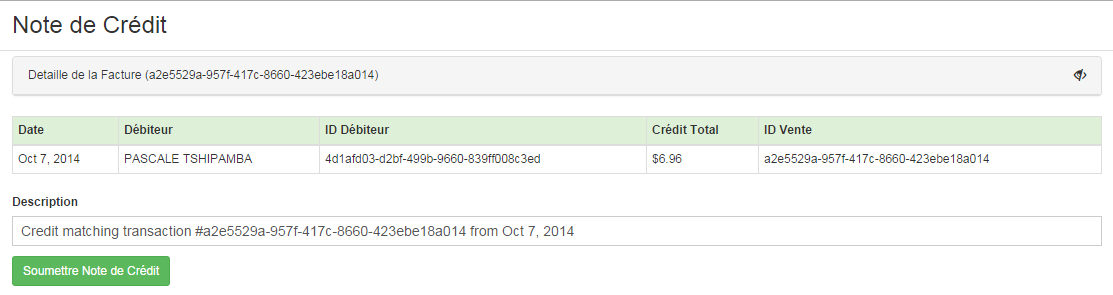
\includegraphics[width=14cm]{pic/NoteCreditMenu.png}
\end{center}
\caption{Interface permettant d'annuler une vente}
\label{Interface permettant d'annuler une vente}
\end{figure}

Pour voir le détaille de la facture il suffit de cliquer sur le bouton 
\includegraphics[scale=0.7]{pic/SeeInvoice.png} qui se trouve dans le coin droit de la zone Détaille de facture   


Et pour annuler une vente il suffit de cliquer sur le bouton 
\includegraphics[scale=0.7]{pic/SubmitNoteCredit.png}  pour que s'affiche sur l'écran l'interface ci-dessous.

\begin{figure}[h]
\begin{center}
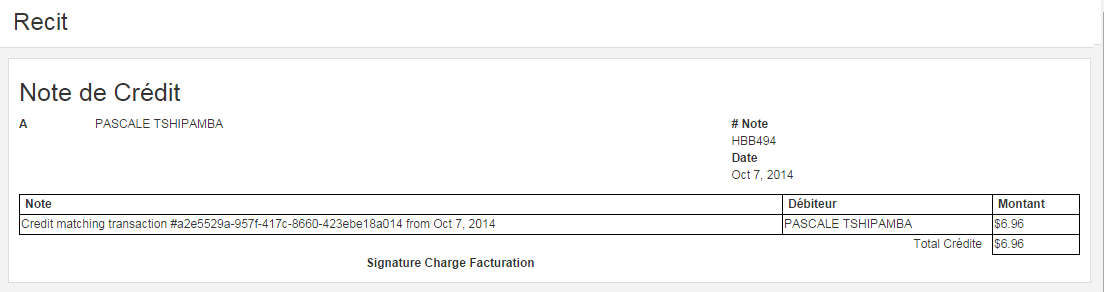
\includegraphics[width=14cm]{pic/RecetteCredit.png}
\end{center}
\caption{Aperçue d'une vente qui a été annulée}
\label{Aperçue d'une vente qui a été annulée}
\end{figure}

Et quand on revient sur la page principale de l'historique de vente on peut se rendre compte que les ventes annulés se colorent différemment des autres, comme on peut le constaté dans la figure ci-dessous.

\begin{figure}[h]
\begin{center}
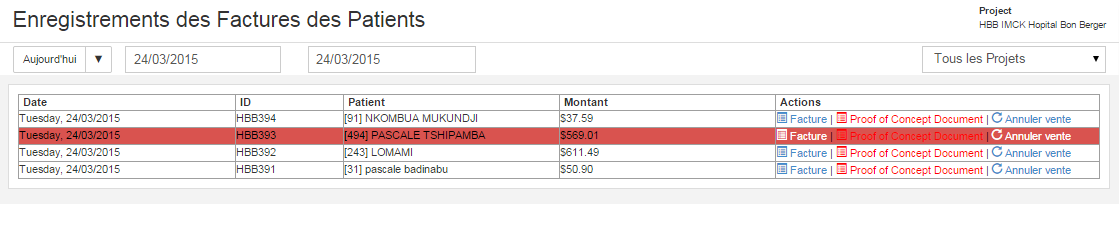
\includegraphics[width=14cm]{pic/HistoriqueVenteDell.png}
\end{center}
\caption{Aperçue de l'historique des ventes avec des ventes annulées}
\label{Aperçue de l'historique des ventes avec des ventes annulées}
\end{figure}

\section{La caisse auxiliaire}
La caisse auxiliaire est un module qui permet le paiement des factures, pour le patient qui sont dans la catégorie \textbf{payant cash}. L'interface principale de ce module se présente comme ceci.


\begin{figure}[h]
\begin{center}
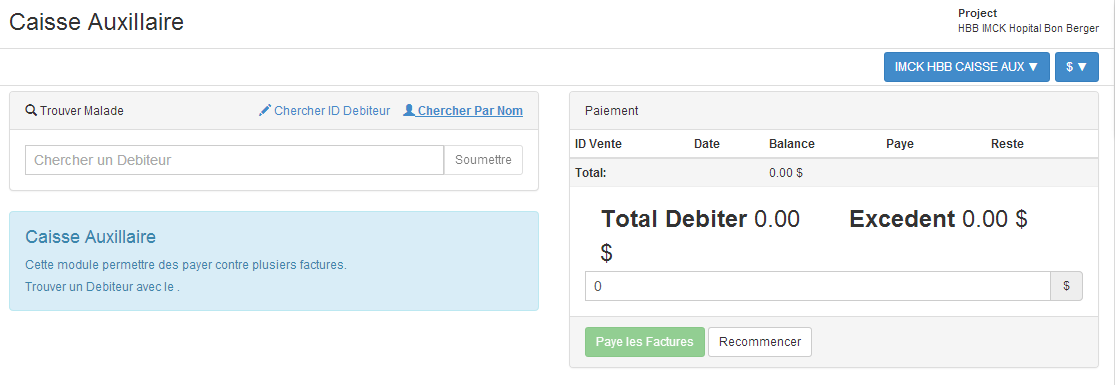
\includegraphics[width=14cm]{pic/CaisseAuxillaire.png}
\end{center}
\caption{Interface principale de la caisse auxilliare}
\label{Interface principale de la caisse auxilliare}
\end{figure}

Dans la partie qui se trouve à droite, on retrouve deux bouton le premier fait référence aux projets et le second fait référence à l'unité monétaire utilisé par le patient pour le paiement de la facture. En dessous de cette zone retrouve la zone qui permet de trouver un patient soit par son \textbf{Id Débiteur} ou bien par son \textbf{Nom}. 
Une fois qu'on a retrouvé un patient et qu'on cliqué sur le bouton soumettre, si ce dernier a des factures à payer ceux-ci s'affiche dans la zone qui se trouve en bas de la zone de recherche. 

\begin{figure}[h]
\begin{center}
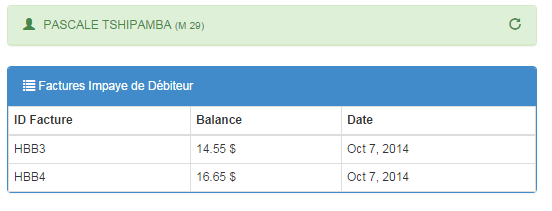
\includegraphics[width=14cm]{pic/ViewInvoice.png}
\end{center}
\caption{Aperçue des factures impayées}
\label{Aperçue des factures impayées}
\end{figure}

Comme le montre l'exemple de la figure ci-haute on peut apercevoir que ce patient a deux factures en attente de paiement. Pour choisir la facture pour laquelle on veut payer il suffit de cliquer sur ça pour que le détaille de ce dernier s'affiche dans la zone qui est juste à droite du tableau \textbf{factures impayé de débiteur}.



\begin{figure}[h]
\begin{center}
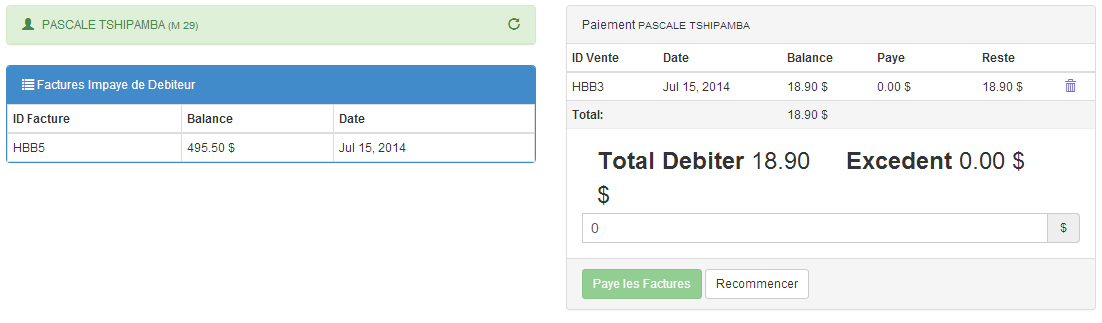
\includegraphics[width=14cm]{pic/PaidInvoice.png}
\end{center}
\caption{Aperçue du processus des paiements des plusieurs factures à la fois}
\label{Aperçue du processus des paiements des plusieurs factures à la fois}
\end{figure}

Sur cette zone on peut distinctement voir le total à payer, il y'a aussi une zone qui permet de saisir le montant payé par le patient ainsi que l'unité monétaire utilisé pour  le paiement. Une fois qu'on a inscrit le montant payé par l'utilisateur on peut cliquer sur le bouton \textbf{payer les factures}.

\begin{figure}[h]
\begin{center}
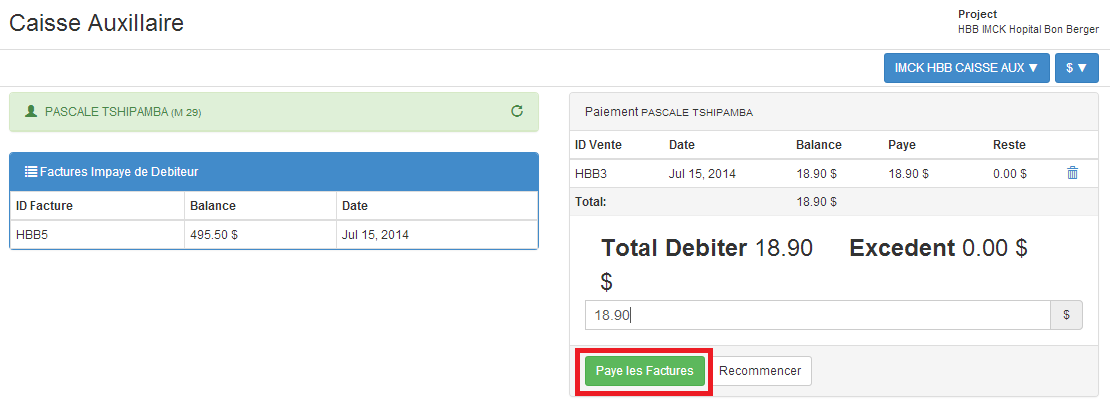
\includegraphics[width=12cm]{pic/PaidInvoiceOK.png}
\end{center}
\caption{Validation du processus de paiement d'une facture}
\label{Validation du processus de paiement d'une facture}
\end{figure}
\newpage
On peut aussi signaler grâce à cet interface, on a la possibilité de payé plusieurs factures à la fois, pour cela il suffit pour cela de choisir ceux dont on voudrait payer, dans la figure qui se retrouve juste après on peut voir l'illustration de ce cas.

\begin{figure}[h]
\begin{center}
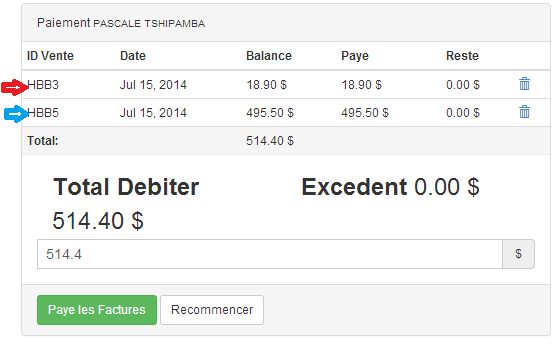
\includegraphics[width=12cm]{pic/PaidDoubleFact.png}
\end{center}
\caption{Validation du processus de paiement des plusieurs factures}
\label{Validation du processus de paiement des plusieurs factures}
\end{figure}
Une fois que le \textbf{bouton payer les factures} est cliqué une facture apparait à l'écran, comme l'illustre la figure ci-après.

\begin{figure}[h]
\begin{center}
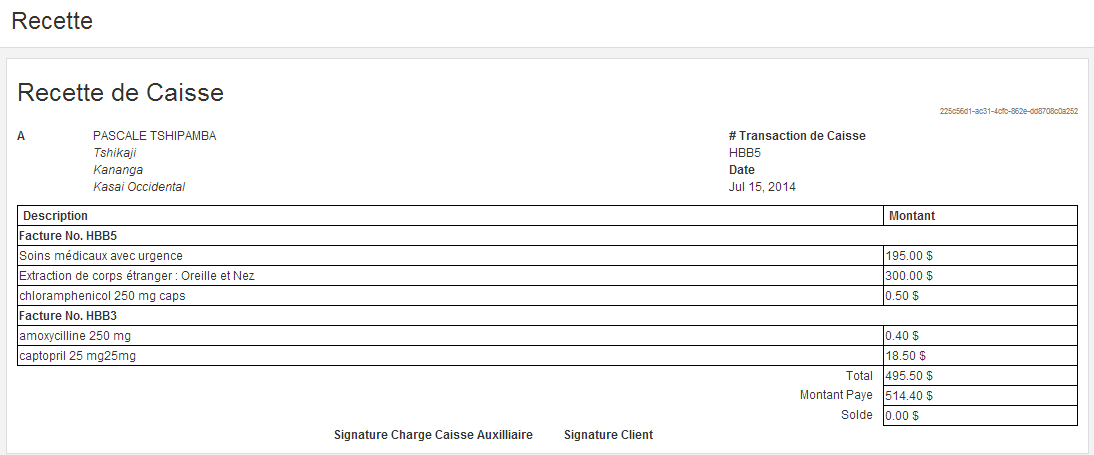
\includegraphics[width=14cm]{pic/FactureDoubles.png}
\end{center}
\caption{Aperçue d'une facture résultant du paiement des plusieurs factures à la fois}
\label{Aperçue d'une facture résultant du paiement des plusieurs factures à la fois}
\end{figure}

\newpage
\section{Facturation des conventions}
Le module facturations des conventions est un modules qui permet à un groupe débiteur de prendre en charge la totalité ou bien une partie de ce que doit un patient à l'hôpital. Son interface d'utilisation se présente de la manière suivante.

\begin{figure}[h]
\begin{center}
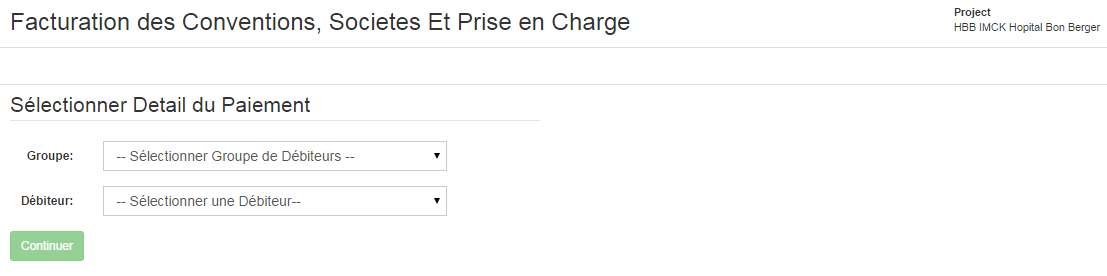
\includegraphics[width=14cm]{pic/FacturationConv.png}
\end{center}
\caption{Interface principale de la facturation des conventions}
\label{Interface principale de la facturation des conventions}
\end{figure}

Quand à l'utilisation de cette interface, il suffit de preciser le groupe débiteur qui accepte de prendre en charge un patient, et en suite recherche le patient en question dans la liste de débiteur, après avoir retrouver le patient en question il faudrait cliquer sut le bouton  \textbf{Continuer} pour faire apparaitre le bouton l'interface qui permet de la prise en charge.

\begin{figure}[h]
\begin{center}
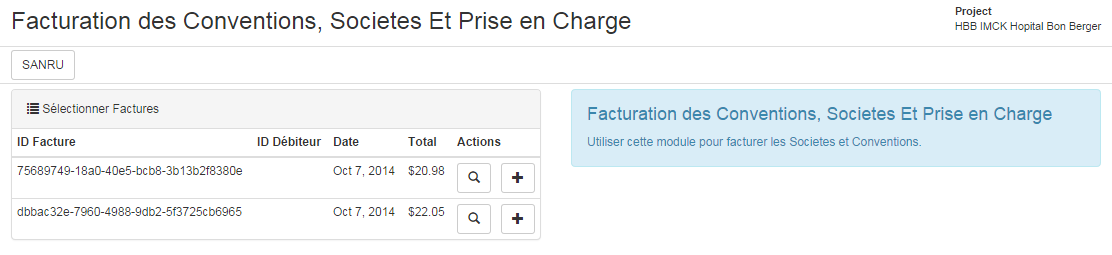
\includegraphics[width=14cm]{pic/FactPrCharge.png}
\end{center}
\caption{Apperçue de l'interface de prise en charge}
\label{Apperçue de l'interface de prise en charge}
\end{figure}

Dans la figure précedante nous pouvons appercevoir une illustration de la prises en charge, dans cette exemple un patient a deux factures en attente de paiement, la zone action possède pour les différentes factures deux icônes 
\includegraphics[scale=0.7]{pic/LoopBlack.png} qui permet d'avoir un aperçue de la facture et 
\includegraphics[scale=0.7]{pic/plusBlack.png} permet d'aller à l'interface permettant la prise en charge proprement dit de la facture. 
Voici l'interface permettant à un débiteur de prendre en charge un patient.

\begin{figure}[h]
\begin{center}
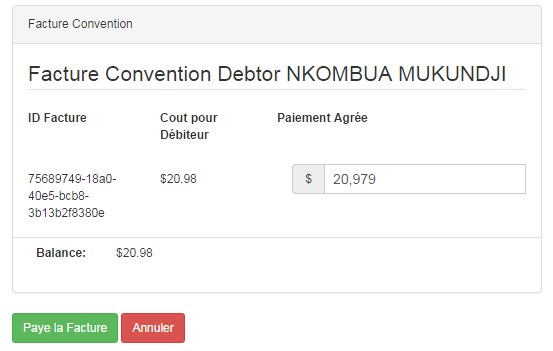
\includegraphics[width=9cm]{pic/FactConv1.png}
\end{center}
\caption{Apperçue de l'interface permettant d'effectue une prise ne charge}
\label{Apperçue de l'interface permettant d'effectue une prise ne charge}
\end{figure}

\begin{figure}[h]
\begin{center}
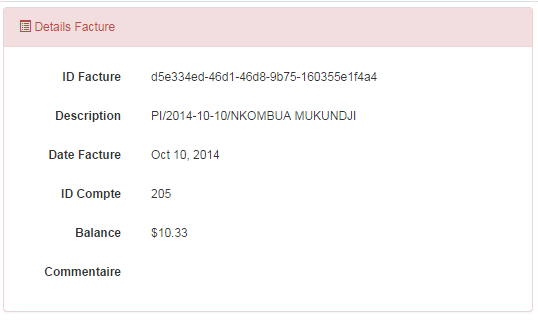
\includegraphics[width=9cm]{pic/DetailConv.png}
\end{center}
\caption{Apperçue d'une facture}
\label{Apperçue d'une facture}
\end{figure}


Cette interface permet de payer le montant de la prise en charge du patient, par défaut le montant à payer se trouve déjà dans la zone de saisie réservée à cet effet 
\includegraphics[scale=0.7]{pic/editableDeb.png}, cette zone de saisie est editable et donne la possibilité de modifier le montant à payer. 

Cet interface permet aussi de prendre en charge plusieur facture appartenant à un même patient en une seul fois, pour cela il suffit simplement de les ajoutant grace à un clic sur l'icône 
\includegraphics[scale=0.7]{pic/plusBlack.png}, et une fois que les factures concernant la prise en charge sont sélectionner, il suffit de cliquer sur le bouton \textbf{Payer la facture} pour être diriger vers une autre interface qui permet de préciser la qui a autorisé le paiement.

\begin{figure}[h]
\begin{center}
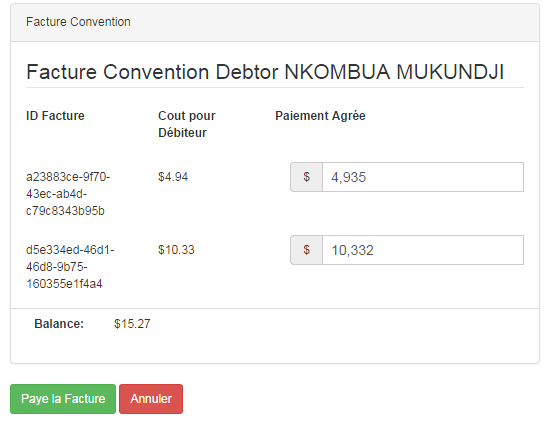
\includegraphics[width=8cm]{pic/DoubleConvention.png}
\end{center}
\caption{Apperçue de l'interface permettant le paiement de deux factures à la fois}
\label{Apperçue de l'interface permettant le paiement de deux factures à la fois}
\end{figure}


\begin{figure}[h]
\begin{center}
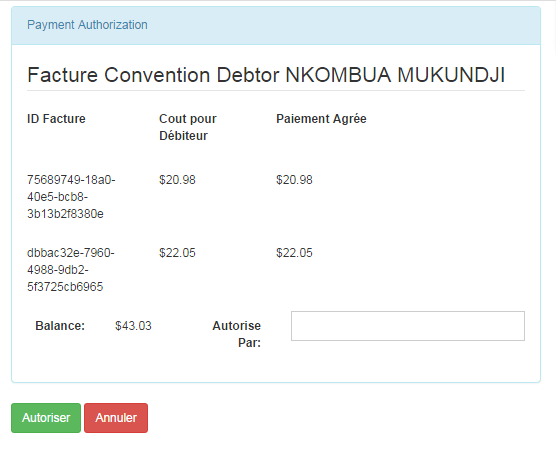
\includegraphics[width=8cm]{pic/PCConfirm.png}
\end{center}
\caption{Apperçue de l'interface permettant de renseigner la personne qui a autorisée le paiement}
\label{Apperçue de l'interface permettant de renseigner la personne qui a autorisée le paiement}
\end{figure}

\newpage
\section{Caution}
Le module Caution est un module qui permet aux patients privés, de pouvoir payer une caution à l'hôpital, cette caution leur donne la possibilité de pour bénéficier des différents services, jusqu'à ce que les motants de la caution s'épuise.

L'interface principale du module gestion de caution se présente de la manière suivante.

\begin{figure}[h]
\begin{center}
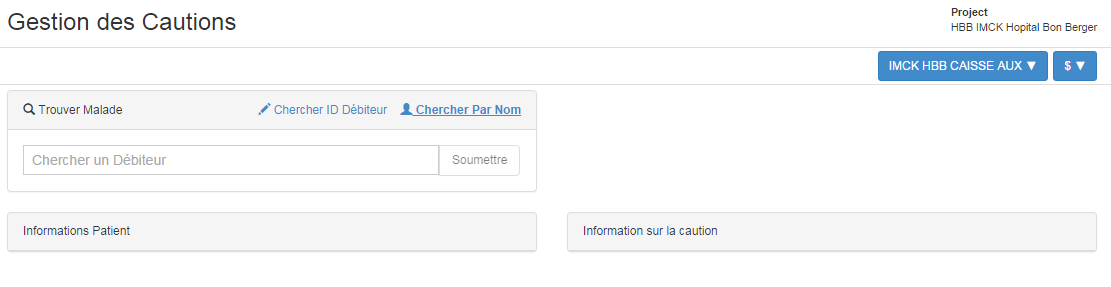
\includegraphics[width=14cm]{pic/cautionInterface.png}
\end{center}
\caption{Interface principale de la gestion des cautions}
\label{Interface principale de la gestion des cautions}
\end{figure}

On retrouve dans le coin droit deux boutons permettant de choisir dans quelle caisse on voudriez payer la caution, mais aussi avec quelle monnaie. 

Il existe aussi la zone qui permet de rechercher le patient. Une fois qu'on a trouver le patient, il ne reste plus qu'à cliquer sur le bouton \textbf{Soumettre} pour que l'interface permettant de payer la caution apparaisse.

\begin{figure}[h]
\begin{center}
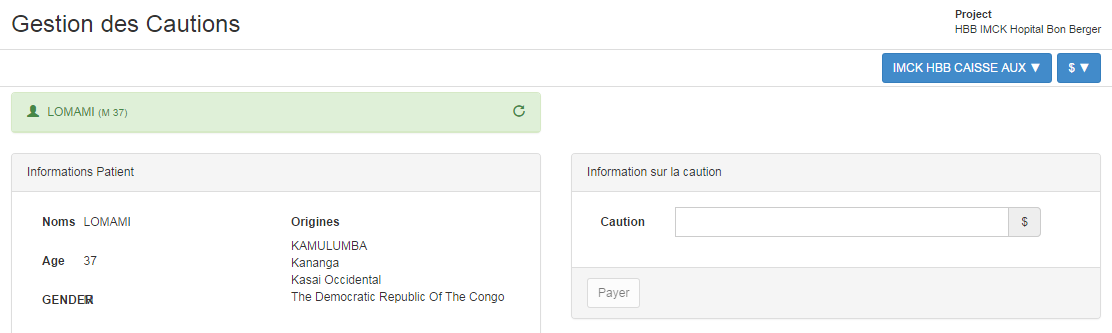
\includegraphics[width=14cm]{pic/formGestionCaution.png}
\end{center}
\caption{Interface principale permettant le paiement d'une caution}
\label{Interface principale permettant le paiement d'une caution}
\end{figure}

Il faudrait saisir dans la zone de saisie qui se trouve dans \textbf{Information de la caution} pour préciser le montant que paie le patient, en suite cliquer sur le bouton Payer, pout permettre la génération du reçu du paiement de la caution.


\newpage
\chapter{Le module Rapports}        
%////////////////////////////////////////////////%
%////////////////////////////////////////////////%
Le module rapports permet de pouvoir visualiser plusieurs types des rapports résultants du fonctionnements du système, La figure ci-dessous représente avec exactitude ce module avec les différents sous éléments.

\begin{figure}[h]
\begin{center}
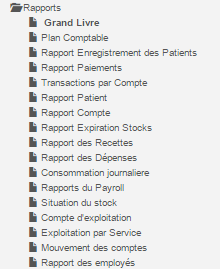
\includegraphics[width=4cm]{pic/ArboReport.png}
\end{center}
\caption{Arborescence du module Rapports}
\label{Arborescence du module Rapports}
\end{figure}

\newpage

\section{Plan Comptable}
Le plan comptable permet la visualisation du plan comptable et donne la possibilité de pouvoit imprimer le plan comptable. L'interface principale de ce module se présente de la manière suivante. 

\begin{figure}[h]
\begin{center}
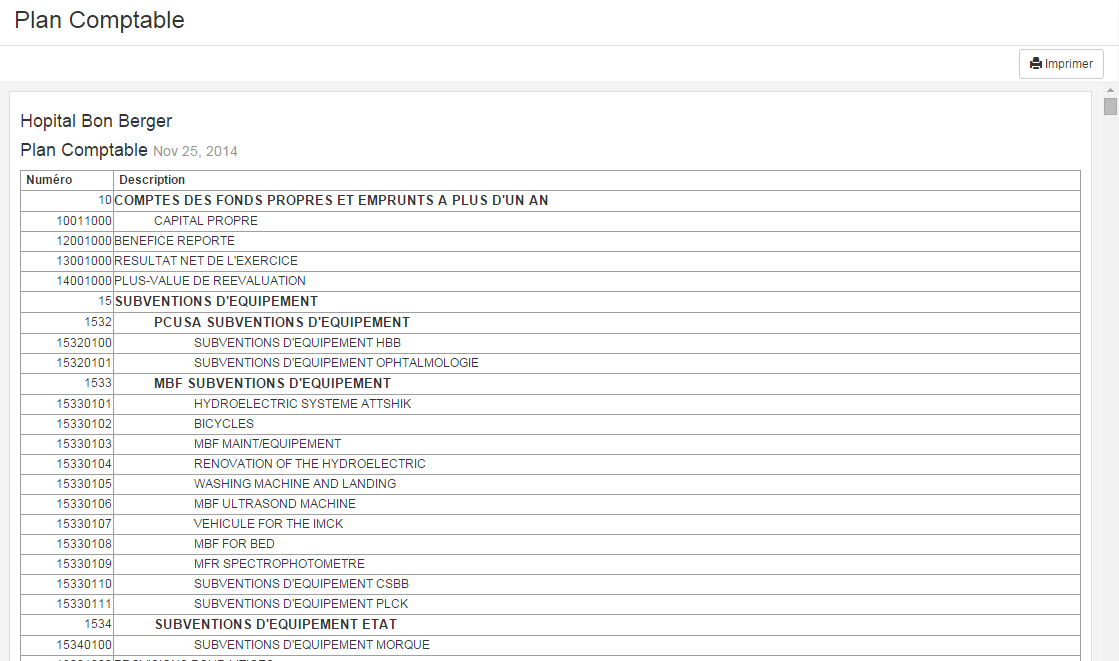
\includegraphics[width=14cm]{pic/PlanComptableAf.png}
\end{center}
\caption{Aperçue du Plan Comptable}
\label{Aperçue du Plan Comptable}
\end{figure}


\newpage
\section{Rapport Paiements}
Le rapport de paiement permet de visualiser l'historique de paiement s'éffectuant aux niveaux des caisses auxilliaires dans le système. L'interface principale permettant de voire le rapport de paiements se présente de la manière suivante. 

\begin{figure}[h]
\begin{center}
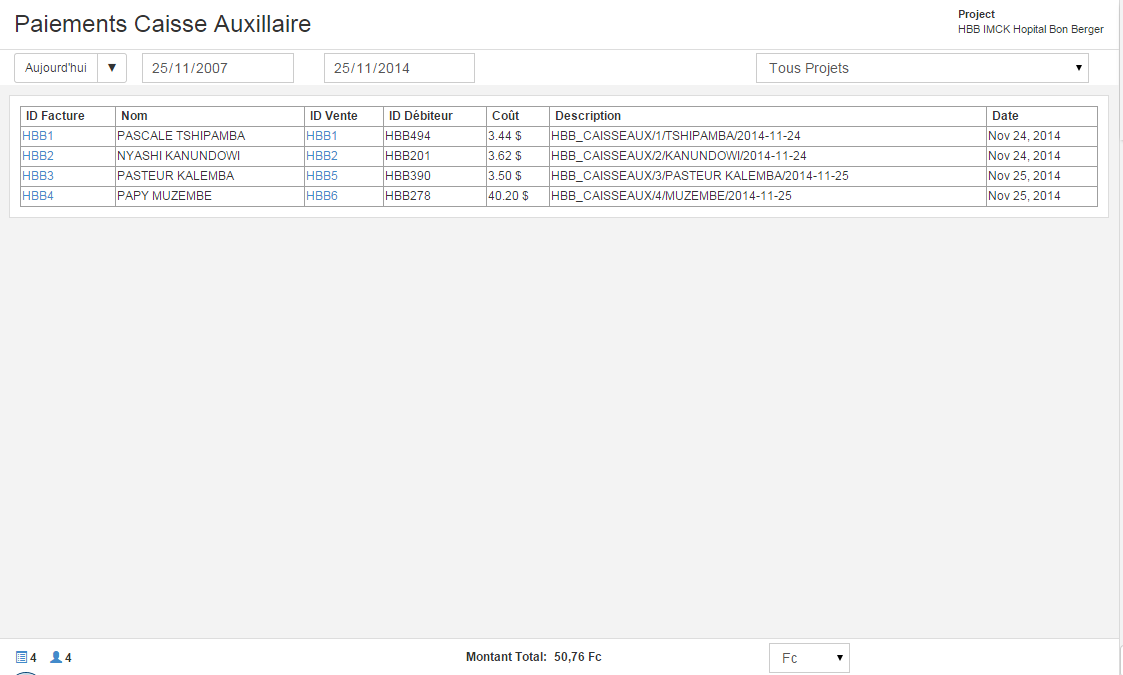
\includegraphics[width=10cm]{pic/rapportCaisseAux.png}
\end{center}
\caption{Aperçue de l'interface principale du rapport de paiements}
\label{Aperçue de l'interface principale du rapport de paiements}
\end{figure}

Par défaut le rapport de paiement affiche la liste des paiements effectués le jour courant, l'interface du rapport d'enregistrement dispose de plusieurs outils permettant de visualiser les anciens paiements répertories.

Le bouton 
\includegraphics[scale=0.7]{pic/Todays.png} donne la possibilité de visualiser les paiements du jour courant, de la semaine courante mais aussi ceux du mois courant. 

Il existe aussi  
\includegraphics[scale=0.7]{pic/PlageTimes.png} qui permet visualiser le rapport de paiement en precisant une plage de valeur entre deux dates.

Il existe aussi une liste de choix qui donne la possibilité de visualiser le rapport d'enregistrement par projets ou bien de tous le projet à la fois.

En bas de page on retrouve les indicateurs sur le rapport de paiements, on retrouve le nombre des paiements qu'il y'a eu ainsi que le montant total des paiements ainsi que la possibilité de visualier le total avec différentes monnaies. 

\begin{figure}[h]
\begin{center}

\includegraphics[width=9cm]{pic/IndRapPaiement.png}
\end{center}
\caption{Aperçue des indicateurs du rapport de paiements}
\label{Aperçue des indicateurs du rapport de paiements}
\end{figure}



%%%%%%%%%%%%%%%%%%%%%%%%%%%%%%%%%%%%%%%%%%%%%%%%%
% Table des matieres
\tableofcontents
\end{document}